\documentclass{article}
\usepackage[T1]{fontenc}
\usepackage{lmodern}
\usepackage{graphicx}
\usepackage{amsmath,amssymb}
\usepackage[a4paper,margin=2cm]{geometry}
\usepackage[absolute,overlay]{textpos}
\setlength{\TPHorizModule}{1mm}
\setlength{\TPVertModule}{1mm}
\usepackage[indonesian]{babel}
\usepackage{hyperref}
\setlength{\emergencystretch}{2em}
% unit: Halaman 16

\begin{document}

% === Halaman 16 (llm) ===

\vspace{112.86mm}

\begin{itemize}
  \item Karena setiap blok plainteks yang sama selalu dienkripsi menjadi blok cipherteks yang sama, maka secara teoritis dimungkinkan membuat buku kode plainteks dan cipherteks yang berkoresponden (asal kata \textit{``code book''} di dalam ECB ). Enkripsi/dekripsi dilakukan dengan \textit{look up table}.
  \vspace{20mm}
  \item Untuk setiap kunci K yang berbeda, dibuat buku kode yang berbeda pula. Jika panjang kunci n bit, maka terdapat $2^n$ buku kode.
\end{itemize}

% deskripsi: Tabel contoh buku kode (look up table) yang memetakan nilai Plainteks ke Cipherteks dalam format biner.
% bbox normalisasi: [0.1300, 0.2900, 0.4300, 0.6700]
\begin{textblock*}{63.00mm}(27.30mm,86.13mm)
\noindent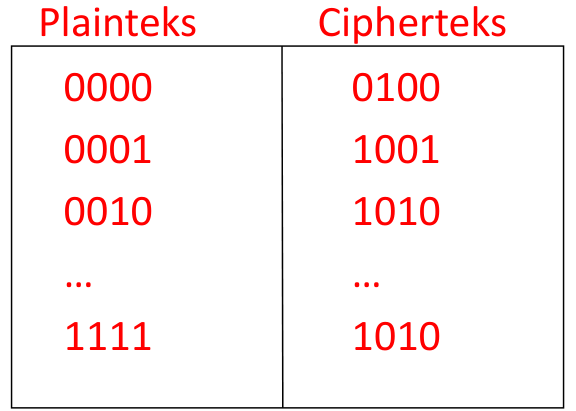
\includegraphics[width=63.00mm,height=112.86mm]{../../images/llm/page_016_img_01.png}%
\end{textblock*}

\end{document}
